\documentclass{article}
\usepackage{tikz}
\tikzset{
  htree leaves/.initial=2,
  sibling angle/.initial=20,
  htree level/.initial={}
}

\makeatletter

\def\htree@growth{%
  \pgftransformrotate{%
    (\pgfkeysvalueof{/tikz/sibling angle})*(-.5-.5*\tikznumberofchildren
      +\tikznumberofcurrentchild)}%
  \pgftransformxshift{\the\tikzleveldistance}%
  \pgfkeysvalueof{/tikz/htree level}%
}
\tikzstyle{htree}=[
  growth function=\htree@growth,
  sibling angle=180,
  htree level={
    \tikzleveldistance=.707\tikzleveldistance
    \pgfsetlinewidth{.707*\the\pgflinewidth}
  }
]

\tikzstyle{btree}=[
  growth function=\htree@growth,
  sibling angle=60,
  htree level={
    \tikzleveldistance=.55\tikzleveldistance
    \pgfsetlinewidth{.707*\the\pgflinewidth}
  }
]

\long\def\ge@addto@macro#1#2{%
  \begingroup
  \toks@\expandafter\expandafter\expandafter{\expandafter#1#2}%
  \xdef#1{\the\toks@}%
  \endgroup}

\newcommand{\htree}[2][]{%
  \def\htree@start{\noexpand\coordinate}
  \def\htree@end{}
  \foreach \l in {0,...,#2} {
    \g@addto@macro\htree@start{child foreach \noexpand\x in {1,2} {\iffalse}\fi}
    \g@addto@macro\htree@end{\iffalse{\fi}}
    \global\let\htree@start\htree@start
    \global\let\htree@end\htree@end
  }
  \edef\htree@cmd{\htree@start\htree@end;}
  \begin{scope}[htree,#1]
  \htree@cmd
  \end{scope}
}

\makeatother

\begin{document}
%\begin{tikzpicture}[
%  rotate=90,
%  yscale=.5,
%  level distance=3cm,
%  line width=8pt,
%]
%\htree{7}
%\htree[btree,yshift=-12cm,xshift=-3cm]{7}
%\end{tikzpicture}

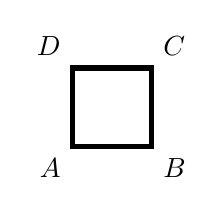
\begin{tikzpicture}[line width=2pt];
  \draw (0,0) node [below left]  {$A$} -- 
        (1,0) node [below right] {$B$} -- 
        (1,1) node [above right] {$C$} -- 
        (0,1) node [above left]  {$D$} -- 
        cycle;
\end{tikzpicture}

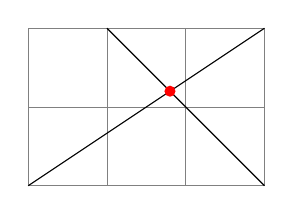
\begin{tikzpicture}
  \draw[help lines] (0,0) grid (3,2);
  \draw (0,0) coordinate (A) -- (3,2) coordinate (B);
  \draw (1,2) -- (3,0);
  \draw (0, 0) coordinate (C);
  \fill[red] (intersection of (0, 0)--(3, 2) and 1,2--3,0) circle (2pt);
\end{tikzpicture}

\tikz{\draw (-1,-1) -- (1,1); \path[fill=green!80!blue,draw=red] (0,0) circle (7mm);}

\tikz{\draw (0,0) --  +(1,0) --  +(0,1) --  +(1,1);}
\tikz{\draw (0,0) -- ++(1,0) -- ++(0,1) -- ++(1,1);}
\tikz{\draw (1,0) -- (0,0) -- (30:1);}
\tikz{\draw (-1, -1) -- (1, 1)  (0, 1) -- (-1, 0)}

te

\pagestyle{empty}
\begin{tikzpicture}[domain=0:4]
    \draw[very thin,color=gray] (-0.1,-1.1) grid (3.9,3.9);
    \draw[->] (-0.2,0) -- (4.2,0) node[right] {$x$};
    \draw[->] (0,-1.2) -- (0,4.2) node[above] {$f(x)$};
    \draw[color=red] plot[id=x] function{x} 
        node[right] {$f(x) =x$};
    %\draw[color=blue] plot[id=sin] function{sin(x)} 
    %    node[right] {$f(x) = \sin x$};
    %\draw[color=orange] plot[id=exp] function{0.05*exp(x)} 
    %    node[right] {$f(x) = \frac{1}{20} \mathrm e^x$};
\end{tikzpicture}




\end{document}